\section{Case Studies and Evaluation}

So far, the Flyspeck project has four core members who collaborate via
GoogleCode\cite{website:FlyspeckProjectPage}.  While the services offered by
GoogleCode (a Subversion repository, a mailing list, and others) were
found to be sufficient for the core development team, we were not
satisfied with the wiki integrated into the GoogleCode web interface.
Lacking support for mathematical formulae, it would not even allow for
presenting the theorems and lemmas to be formally proven in a
human-readable fashion.  Furthermore, GoogleCode offers very
little \emph{structuring} support, which we believe will be
essential for browsing and querying Flyspeck's 
(eventually) large knowledge collection.  We sought to improve
on GoogleCode with two prototypes.  
In the following sections, we evaluate the prototypes 
for their applicability to Flyspeck with regard to their
support for annotations, browsing, and querying, as specified in
section~\ref{sec:req}.  For the case study, we took a simplified 
view of Flyspeck, using only the {\TeX} sources of the
Flyspeck book and a Twelf formalization of the first chapter (Trigonometry).
The goal was to present the trigonometry chapter in a compelling way
that we believed would scale 2-3 orders of magnitude.  

Both systems are semantic wikis, where one resource (in the RDF sense)---e.\,g.\
one mathematical theorem---is represented by one wiki page and relations between
resources by links between pages.  Both pages and links can be typed with terms
from ontologies\cite{OrDeMoVoHa06:annotation-navigation-semwiki}, which are
either preloaded into the wiki or modelled
ad-hoc\cite{KrSchVr:semwiki-reasoning07}.  This is the prevalent approach of
adding semantics to wikis, although other ways have been
investigated\cite{semwiki06}.  Semantic wikis offer enhanced navigation
capabilities.  For example, they can usually display a summary of all typed
links, grouped by type, for each page.  They support searching for pages by type
or by a page being source or target of a typed link\footnote{Both explicit and
  inferred links (= RDF triples) can be
  considered\cite{KrSchVr:semwiki-reasoning07}}.  Such queries can usually be
executed interactively, or in an automated way as \emph{inline} queries embedded
into the content of a page\cite{KrSchVr:semwiki-reasoning07}.  Both systems we
consider support this basic set of semantic wiki features.

\subsection{Semantic MediaWiki 1.0}
\label{sec:smw-study}

Semantic MediaWiki\cite{KrSchVr:semwiki-reasoning07} is a semantic web extension
to MediaWiki, the system driving \product{Wikipedia}.  Plain MediaWiki supports
mathematical formulae written in {\LaTeX} and allows for categorizing pages.
Semantic MediaWiki interprets category membership as an instance-of relationship
and supports the creation and editing of typed links (called properties).
External ontologies can be referenced from the wiki, but at most sites powered
by Semantic MediaWiki, site-specific ontologies are developed in an ad-hoc
manner\cite{ontoworld:sites-using-smw}.

\paragraph{Prototype} In Semantic MediaWiki, we imported the Twelf master source
of Flyspeck via a customly implemented special page.  The Twelf file was first
enhanced by special comment lines marking the beginning and end of a declaration
with information about topical categorization.  The Twelf upload special page
handler breaks an uploaded file down into declarations and creates two wiki
pages for each Twelf declaration: one page that just contains the Twelf listing,
categorized in the OMDoc document ontology (e.\,g.\ \textit{Lemma}; see
section~\ref{sec:swim}), and one container page that includes the Twelf page via
MediaWiki's template inclusion mechanism, but also allows for including a
{\LaTeX} representation and leaves space for free-form annotations made by the
contributors.  Additionally, MediaWiki offers a discussion page for each page of
mathematical content.  The Twelf pages are overwritten on every import from the
master source, whereas existing container pages remain untouched.  This allows
one to change the computerized version of a Twelf constant in the master source
(e.\,g.\ if it is incorrectly specified) and reimporting it without losing the
semantic markup and comments.

As a first step, we encoded the types of knowledge items in the identifier of
the declarations.  For example, the identifier of a lemma would start with
``lemma-''.  We could also have employed Twelf's inference to determine the
type\ednote{@Florian: Reword this correctly! Do you get the idea; is this
  possible?}, as our existing Twelf-to-OMDoc converter does.  Additionally, the
upload extension recognizes all previously imported symbols in Twelf expressions
and turns them into links of the type \textit{\ldots--uses--Symbol}.

\begin{figure}
  \centering
  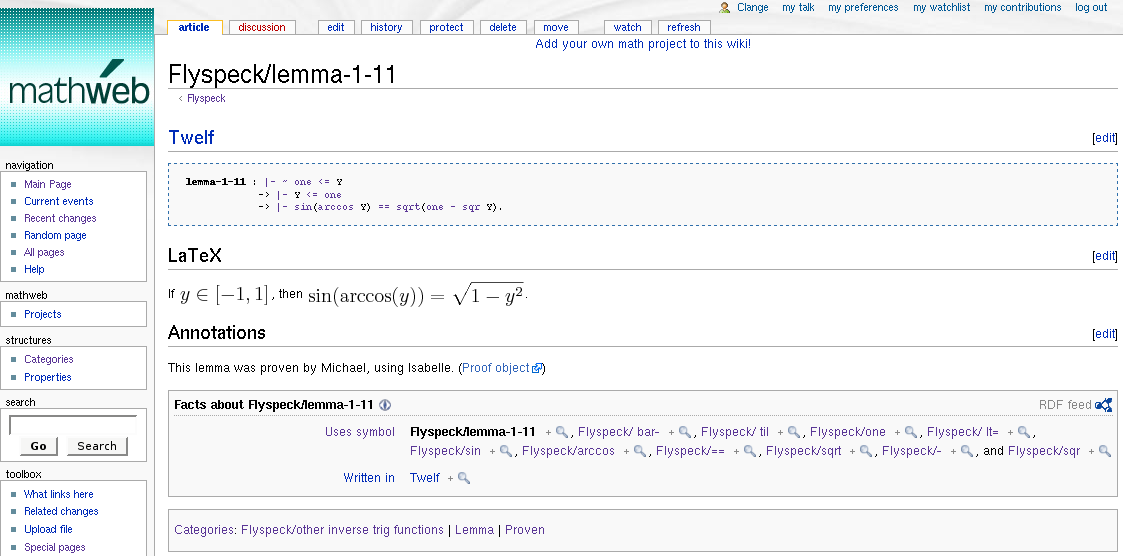
\includegraphics[width=\textwidth]{images/smw-lemma}
  \caption[A Flyspeck lemma in Semantic MediaWiki]{A Flyspeck lemma in Semantic
    MediaWiki\protect\footnotemark}
  \label{fig:smw-lemma}
\end{figure}
\addtocounter{footnote}{-1}
\stepcounter{footnote}\footnotetext{See \url{http://mathweb.org/wiki/Flyspeck}}

The annotations generated that way can be used for browsing, either via the
``fact box'' (the summary of all typed links), or by the special ``browse''
page.  For querying, Semantic MediaWiki offers a simple triple search, as well
as inline queries.  The query language corresponds to the description logic
$\mathcal{EL}^{++}$\cite{KrSchVr:semwiki-reasoning07}, which, for example, does
not support negation.  A query for unproven lemmas about a certain topic could
only be performed if the ``unprovenness'' were explicitly annotated.  The
following queries additionally ask for lemmas available in a Twelf formalization:

\begin{lstlisting}
<ask>[[Category:Unproven]] [[Category:Lemma]]
     [[Category:Trigonometry]] [[written in::Twelf]]</ask>
\end{lstlisting}

Exporting computerized representations of knowledge items is not yet supported
conveniently.  The Twelf listings can be viewed on their own pages, but due to
the auto-generated symbol links in the source code, these are not suitable for
download.  One would either have to implement a special Twelf download page that
cleans these sources again, or one would have to implement the symbol linking as
an extension of the rendering process.

\paragraph{Evaluation} We found the ad-hoc ontology development useful while
prototyping the annotations that might be required for Flyspeck, e.\,g.\
project-related metadata like the information whether a lemma has already been
proven, or categorization by topic.  Semantic MediaWiki did not meet the
requirements in places where ontologies already existed.  For example, in
structures of mathematical documents, it was possible to reference
\emph{vocabulary} from the OMDoc document ontology, but not to apply further
inference rules given there to items of mathematical knowledge.  This is because
Semantic MediaWiki does not support a full \emph{import} of external ontologies.
Most annotations were modelled by categorization, i.\,e.\ instantiation of
classes---certainly not the most formal way of structuring knowledge in view of
many classes just corresponding to narrative sections of the book, but the one
that is supported best by Semantic MediaWiki.

Semantic MediaWiki does not understand the semantics of mathematical formulae,
as the {\LaTeX} formulae cannot be annotated.  The Twelf listings could be
annotated, but at the cost of making them harder to download.

The inline queries were intuitive to write but not as powerful as required.
Complex reasoning tasks like inference of dependencies are not possible in
Semantic MediaWiki; in the restricted domain-specific setting of Flyspeck one
could realize them by hard-coded extension functions.

\subsection{SWiM 0.2}
\label{sec:swim}

SWiM is a semantic wiki targeted at mathematical knowledge management.  Based on
the general-purpose semantic wiki
\product{IkeWiki}\cite{KrSchVr:semwiki-reasoning07}, it adds support for
browsing, editing, rendering, importing and exporting mathematical documents
written in OMDoc.  The semantics of mathematical knowledge is mainly captured in
the OMDoc markup, and more explicitly in a \emph{document ontology}: Whenever a
wiki page containing OMDoc fragments is saved, its type and its (typed)
relations to other items of mathematical knowledge in the wiki are extracted
from the OMDoc XML markup and explicitly represented as RDF triples using terms
of the OMDoc document ontology\cite{OMDocDocOnto:web}.  This ontology models
those aspects of the three layers of mathematical knowledge supported by OMDoc
to the extent supported by the expressivity of OWL-DL\cite{McGvHa:owl04}.
Modeling all modules of the OMDoc specification in this ontology is work in
progress; so far, most mathematical statements as well as key aspects of
theories have been implemented.  Relevant classes for Flyspeck would be
\textit{Lemma}/\textit{Theorem}/\textit{Corollary}/\ldots (all being subclasses
of \textit{Assertion}), \textit{Proof}, \textit{Symbol} (a symbol declaration),
\textit{Definition}, and the properties \textit{Proof--proves--Assertion} and
\textit{Symbol--hasDefinition--Definition}.

\begin{figure}
  \centering
  \begin{tikzpicture}[set style={{default}+=[xscale=.5,yscale=.47,font=\normalsize\sffamily]},default]
    \tikzstyle{every path}=[font=\small\sffamily];
    \node[concept] (s) at (0,0) {\itshape Statement};
    \node[concept] (d) at (-7.5,-2.75) {Definition};
    \node[concept] (y) at (-2.5,-2.75) {Symbol};
    \node[concept] (a) at (+2.5,-2.75) {Assertion};
    \node[concept] (p) at (+7.5,-2.75) {Proof};

    \node[concept] (l) at (-1.5,-5) {Lemma};
    \node[concept] (c) at (+2.5,-5) {Corollary};
    \node[concept] (t) at (+6.5,-5) {Theorem};

    \draw[-open triangle 60] (y) -- (s);
    \draw[-open triangle 60] (d) -- (s);
    \draw[-open triangle 60] (a) -- (s);
    \draw[-open triangle 60] (p) -- node[right=1ex] {$\sqsubseteq$} (s);

    \draw[-open triangle 60] (l) -- (a);
    \draw[-open triangle 60] (c) -- (a);
    \draw[-open triangle 60] (t) -- (a);

    \draw[->] (d) -- node[below] {uses} (y);
    \draw[->] (a) -- node[below] {uses} (y);
    \draw[->] (p) -- node[below] {proves} (a);

    \draw[->] (s.0) .. controls +(0:2cm) and +(60:2cm)
    .. node[right=1pt,text width=2cm,text centered] (dep)
    {\itshape depends on} (s.60);

    \draw[->] (y.-120) .. controls +(-120:1cm) and +(-60:1cm) .. node[below] {hasDefinition} (d.-60);
  \end{tikzpicture}
  \caption{A relevant subset of the OMDoc document ontology}
  \label{fig:doconto}
\end{figure}

In the current version 0.2 of SWiM, the browsing of mathematical documents is
powered by the document ontology: Whenever RDF triples having the current page
as subject or object are available, most of them using terms from the OMDoc
document ontology if the current page is a mathematical document, the
\product{IkeWiki} user interface can display them as navigation links (see
figure~\ref{fig:swim-lemma}) or in a graph view.  More ontology-powered
services, particularly ones that facilitate editing documents, are planned for
version 0.3\cite{swim-roadmap,Lange:SWiMSciColl07}.  Documents are presented as
XHTML+MathML, with mathematical symbols linked to their declarations.

\begin{figure}
  \centering
  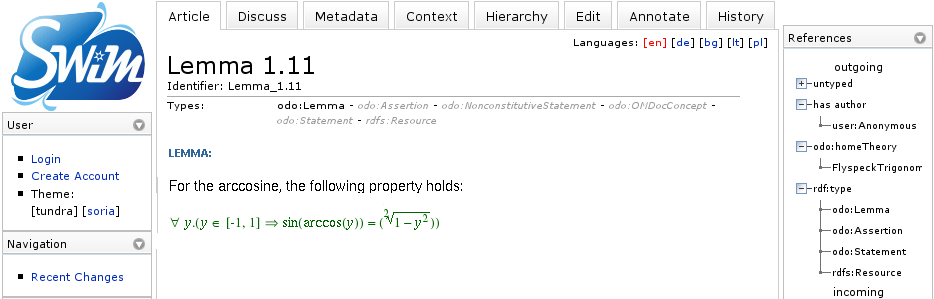
\includegraphics[width=\textwidth]{images/swim-lemma}
  \caption{A Flyspeck lemma in SWiM}
  \label{fig:swim-lemma}
\end{figure}

\paragraph{Prototype} We manually converted part of the trigonometry lemmas to
OMDoc for SWiM (see fig.\ \ref{fig:swim-lemma})\ednote{FYI: Actually only one,
  but we wouldn't have gained more from converting more of them.}  Additionally,
we can auto-generate OMDoc documents from the Twelf source with a converter and
import them into SWiM using the built-in import functionality.

As every SWiM page has an associated discussion page and discussion posts are
semantically represented using the SIOC ontology\cite{SIOC:web}, one can support
the coordination of the project by queries like query~\ref{item:question-count}
from section~\ref{sec:req}.  Work on determining a relevant subset of OMDoc and
its document ontology for discussions is currently in progress\ednote{FYI,
  Florian, this is not a lie but what panta rhei does ;-)}.  Pages and non-OMDoc
links can be annotated with types from ontologies loaded into the
wiki\footnote{Types of OMDoc links are automatically extracted from the markup;
  see above.}.

Authors can embed inline SPARQL queries into wiki pages.  Not all desirable
queries are easy to express in SPARQL; consider query~\ref{item:proven-lemma}:

\begin{lstlisting}
SELECT ?l WHERE { ?l rdf:type odo:Lemma .
                  ?l swrc:isAbout <Composite_Regions> .
                  OPTIONAL { ?p rdf:type odo:Proof .
                             ?p odo:proves ?l . }
                  FILTER ( ! bound(?p) ) }
\end{lstlisting}

This query assumes a SPARQL semantics with negation as
failure\cite{Polleres:SPARQL-Rules07}.

As OMDoc supports all degrees of formalizing mathematical knowledge,
computerized data can be downloaded in their OMDoc representation using SWiM's
export feature and then be converted to Twelf by client-side
software\cite[chap.\ 25.2]{Kohlhase:omdoc1.2}.

\paragraph{Evaluation} Annotating mathematical structures with SWiM is easy---it
just means using the editor and having the annotations extracted.  Other
annotations required for Flyspeck, such as categorizations or progress
information, can be made, but not in an ad-hoc way, which we would have found
useful in the prototyping phase.  Instead, one would have to import an existing
ontology into the wiki, or create it using the build-in ontology editor, and
then one would be able to annotate documents using terms from that ontology.

Browsing is well supported, with incoming and outgoing links being offered for
navigation, and a graphical view of the neighborhood of the current resource in
the RDF graph.

Queries are powerful but not always short and intuitive (see above), but
alternatively, one could just enhance the ontology, harness the power of the
integrated \product{Pellet} OWL-DL reasoner
(see~\cite{KrSchVr:semwiki-reasoning07}), and get the same result with a simple
query for instances of a specially defined class.  For unproven lemmas, the
following axiom would do the trick:

\[
\mbox{LemmaWithoutProof}\equiv\mbox{Lemma}\sqcap\neg(\exists\mbox{proves}^{-1}.\mbox{Proof})
\]

Dependencies can partly be inferred by a DL reasoner, but for a complete support
of OMDoc's notion of dependency, an OMDoc-specific calculus will have to be
applied, which is currently in development.

%%% Local Variables: 
%%% mode: latex
%%% TeX-master: "flyspeck-wiki-eswc08"
%%% End: 
